\documentclass{article}
\usepackage[left=1cm, right=1cm, top=1cm, bottom=1cm]{geometry}
\usepackage{mdframed}
\usepackage{minted}
\usepackage{graphicx}
\usepackage{amsmath}
\usepackage{amstext}
\usepackage{float}
\begin{document}

\title{HA2 Efficient Computing}
\author{Daniel Schicker}
\date{\today}

\maketitle
\section{Improvement factors for different technologies}

\begin{figure}[h]
    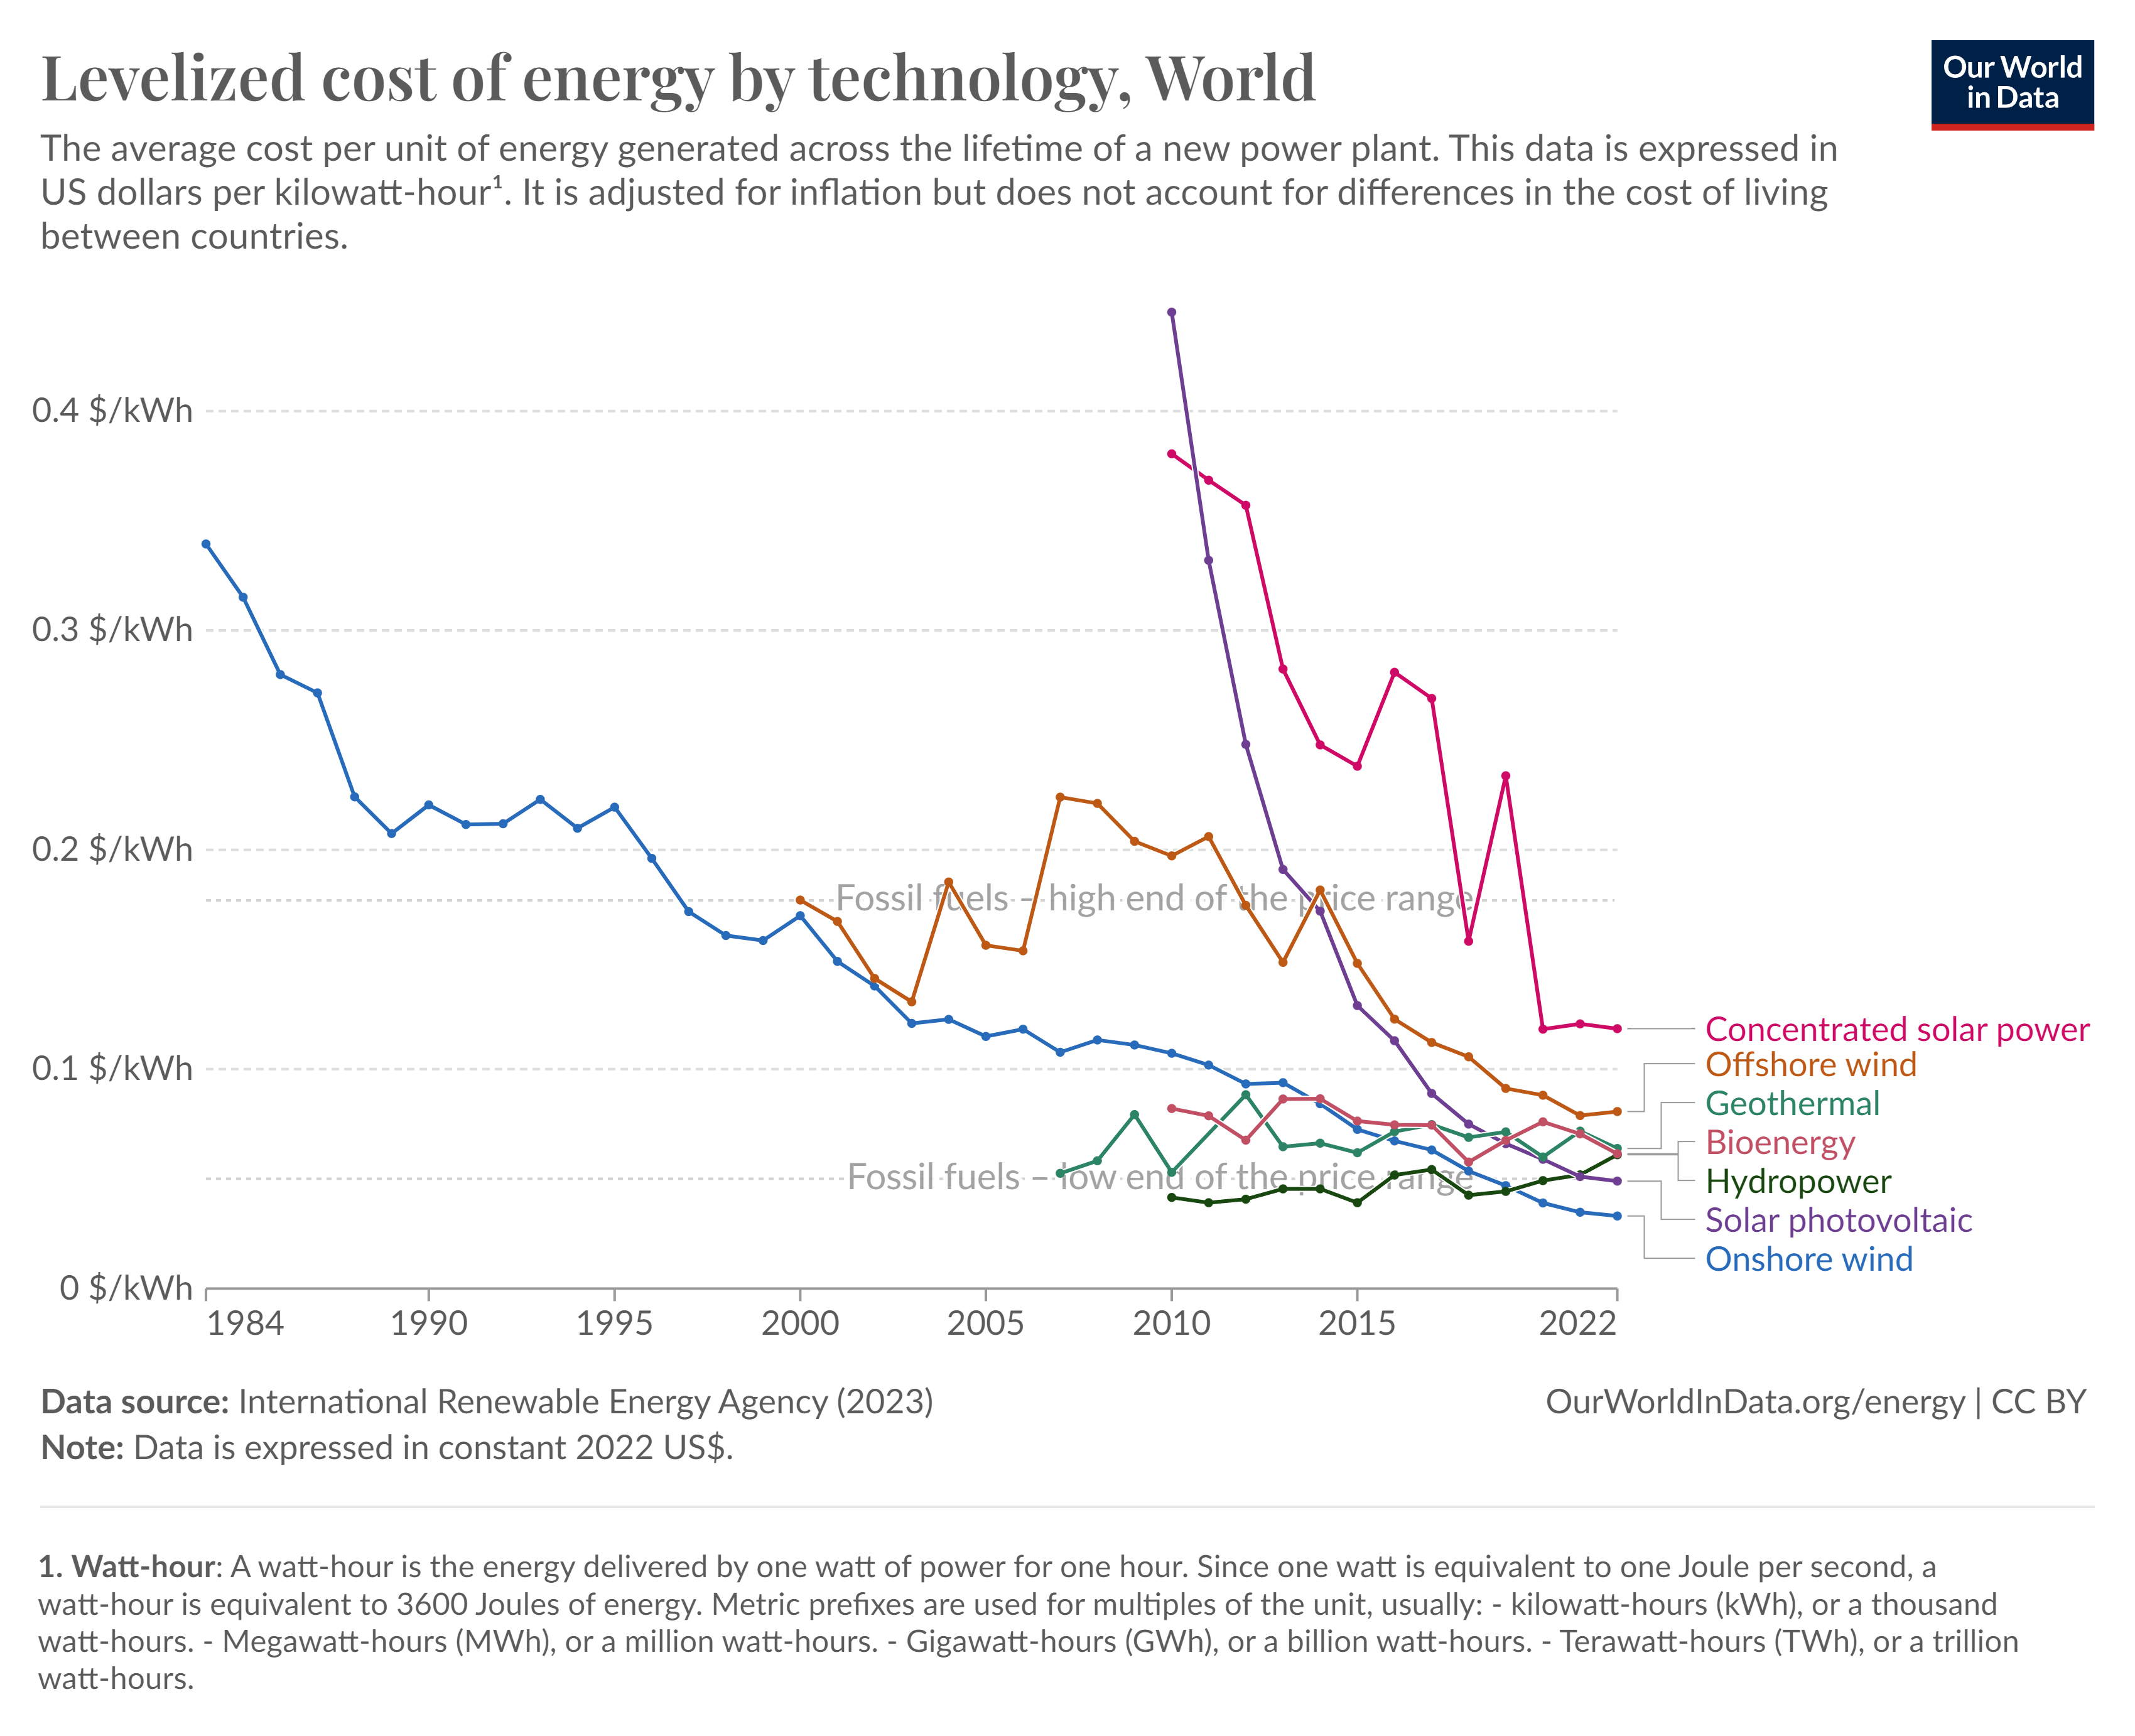
\includegraphics[width=0.8\textwidth]{levelized_cost_of_energy.png}
\end{figure}

\begin{figure}[H]
    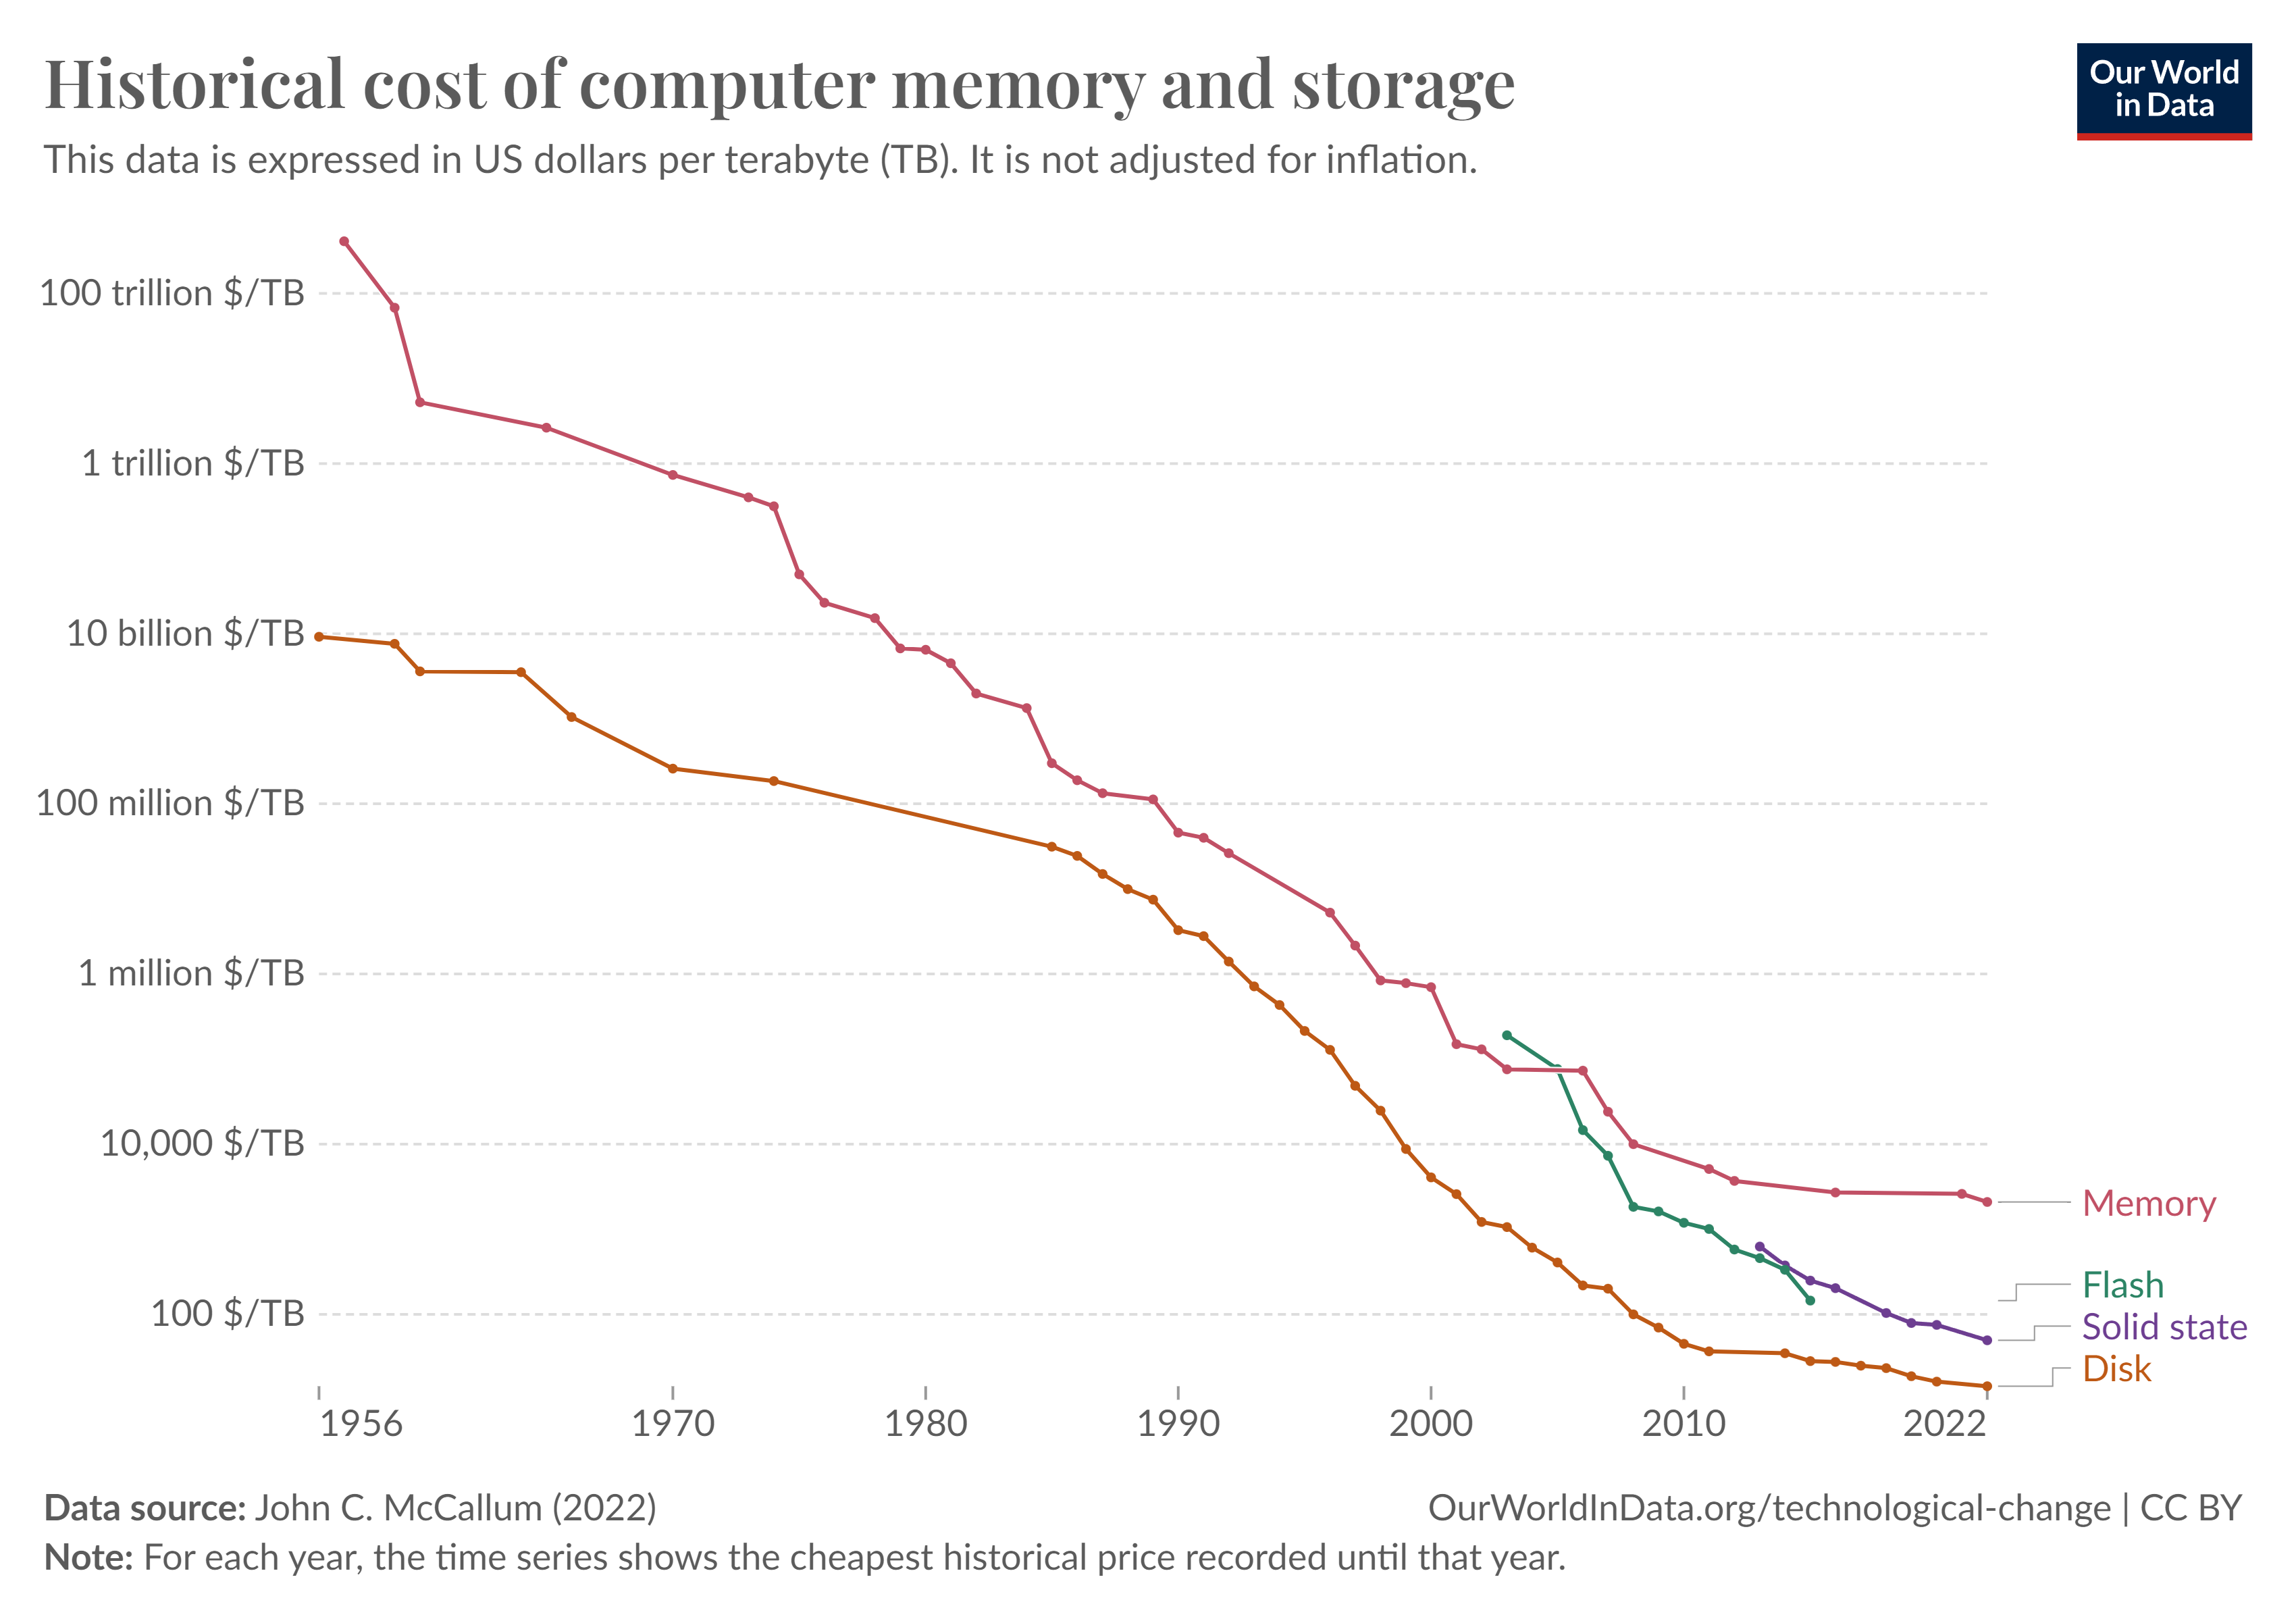
\includegraphics[width=0.8\textwidth]{historical-cost-of-computer-memory-and-storage.png}
\end{figure}

\begin{figure}[H]
    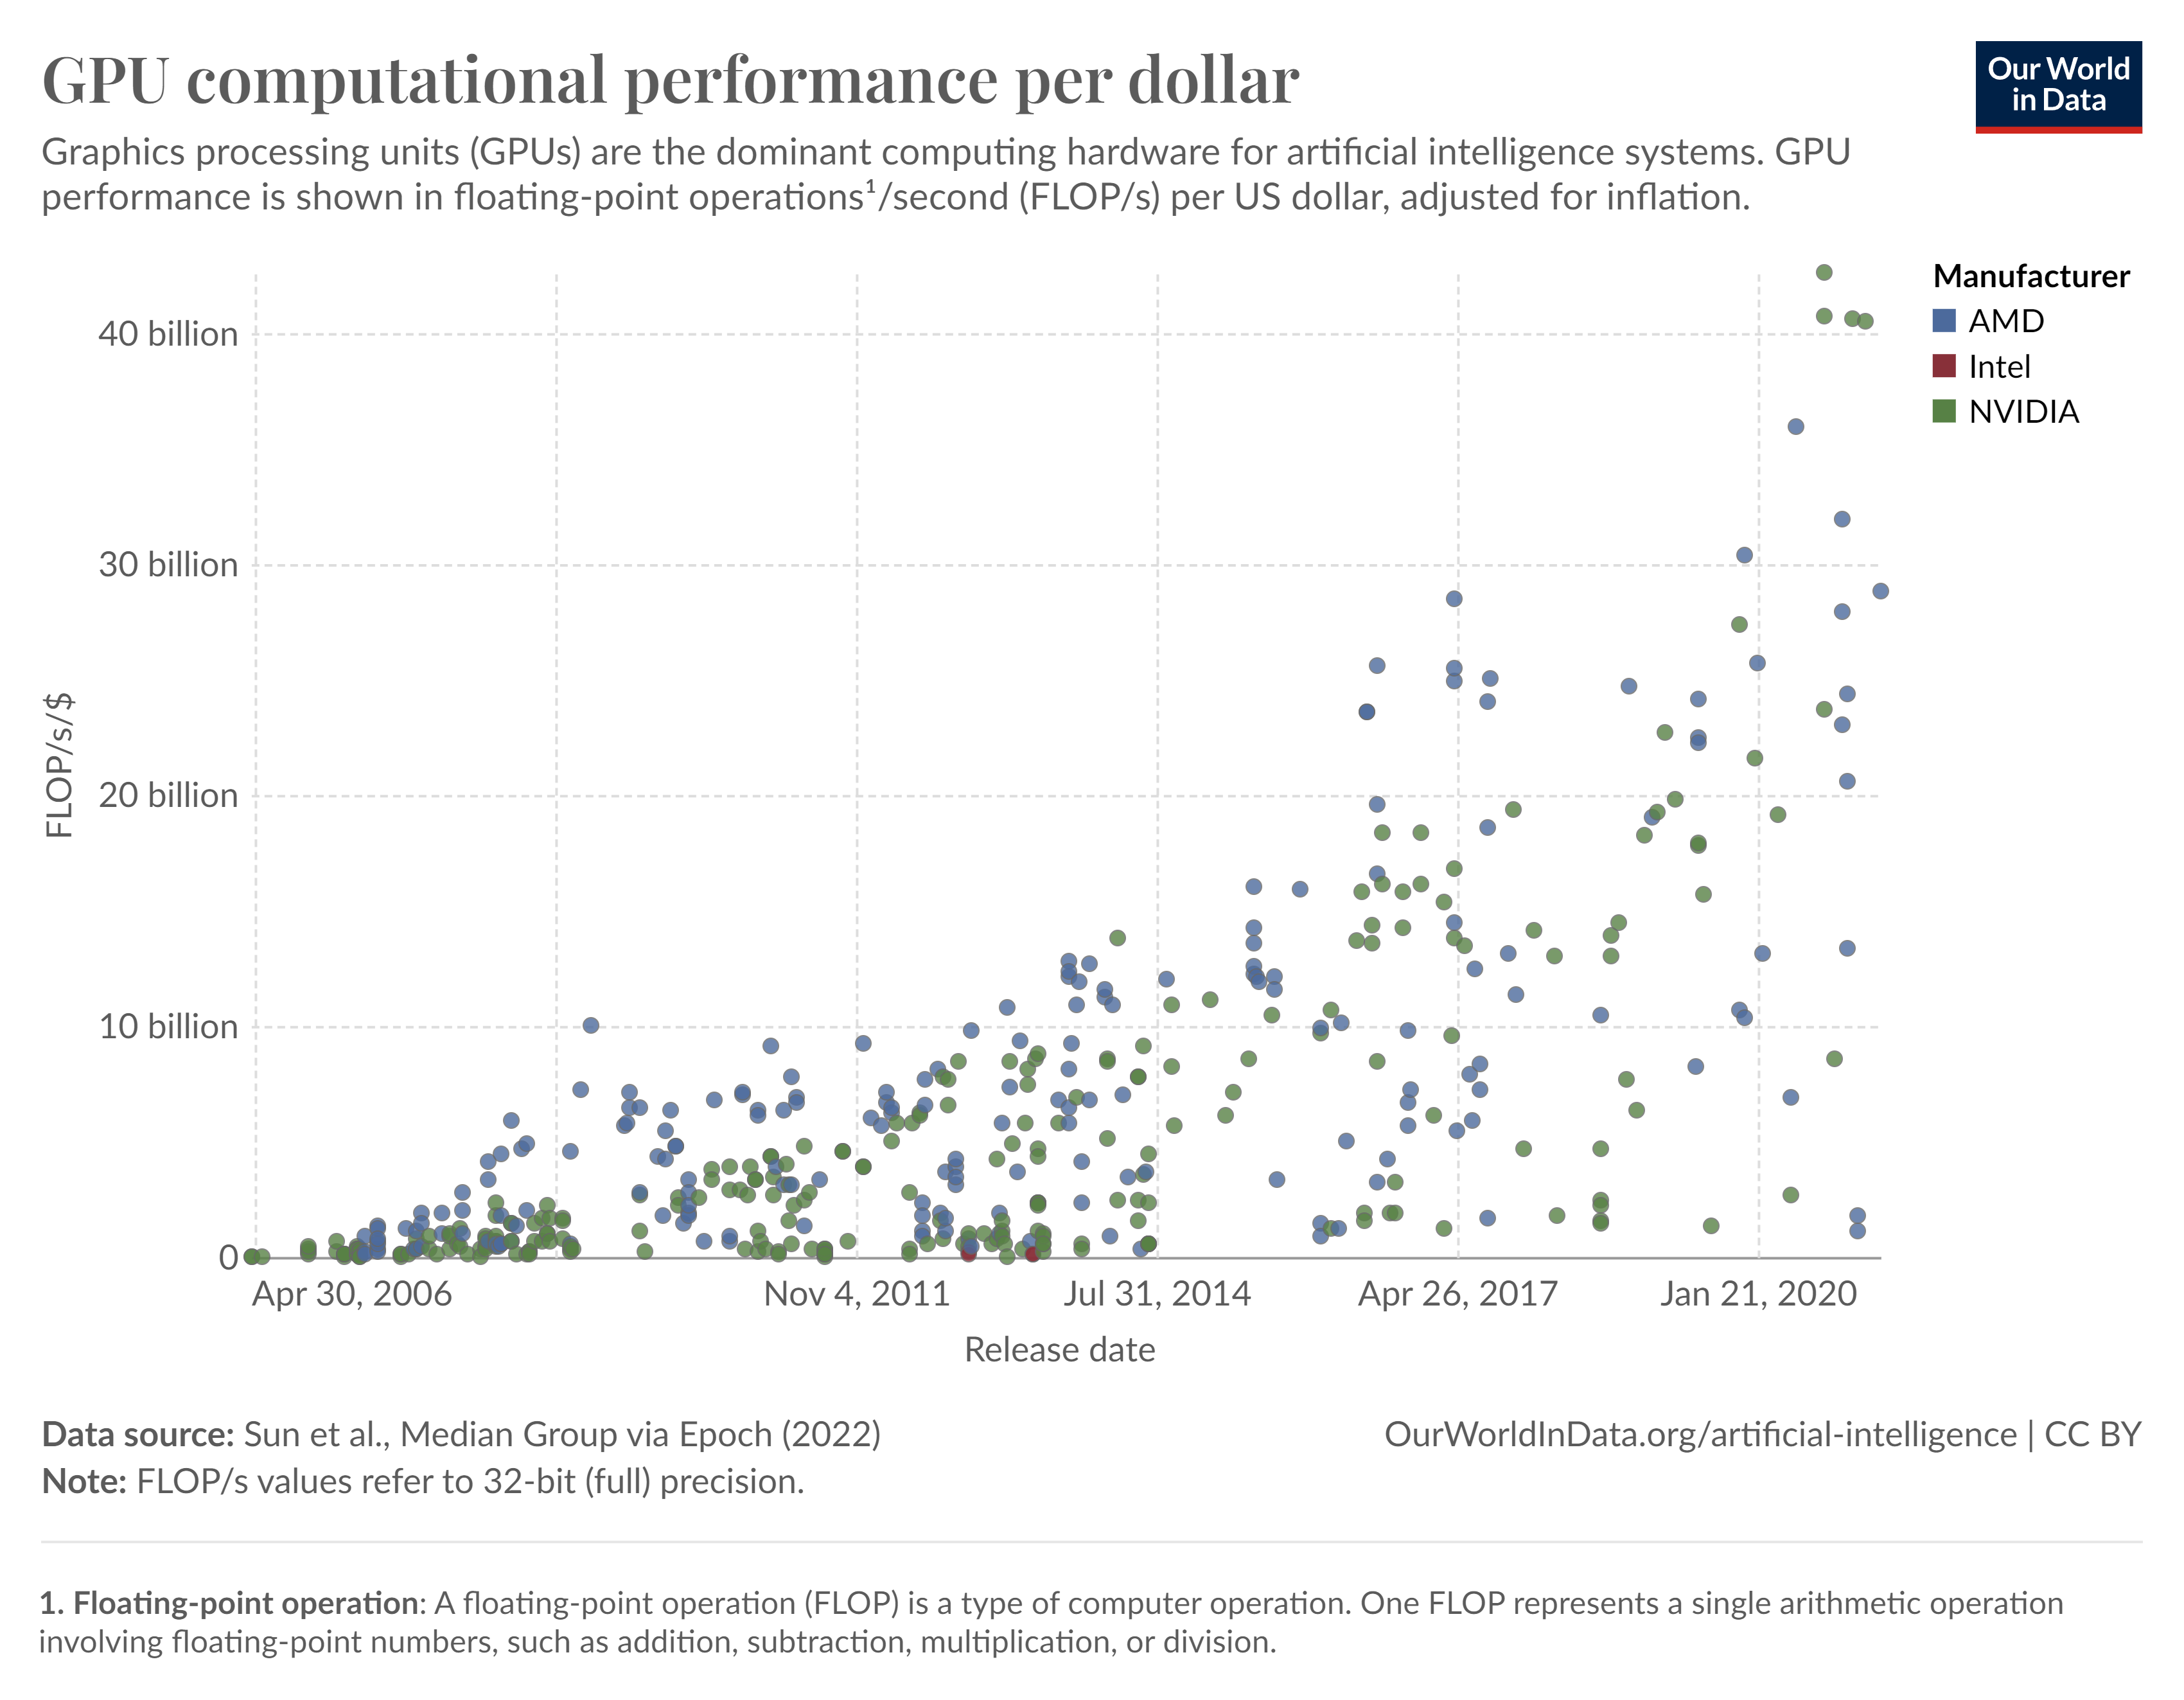
\includegraphics[width=0.8\textwidth]{gpu-price-performance.png}
\end{figure}

\begin{figure}[H]
    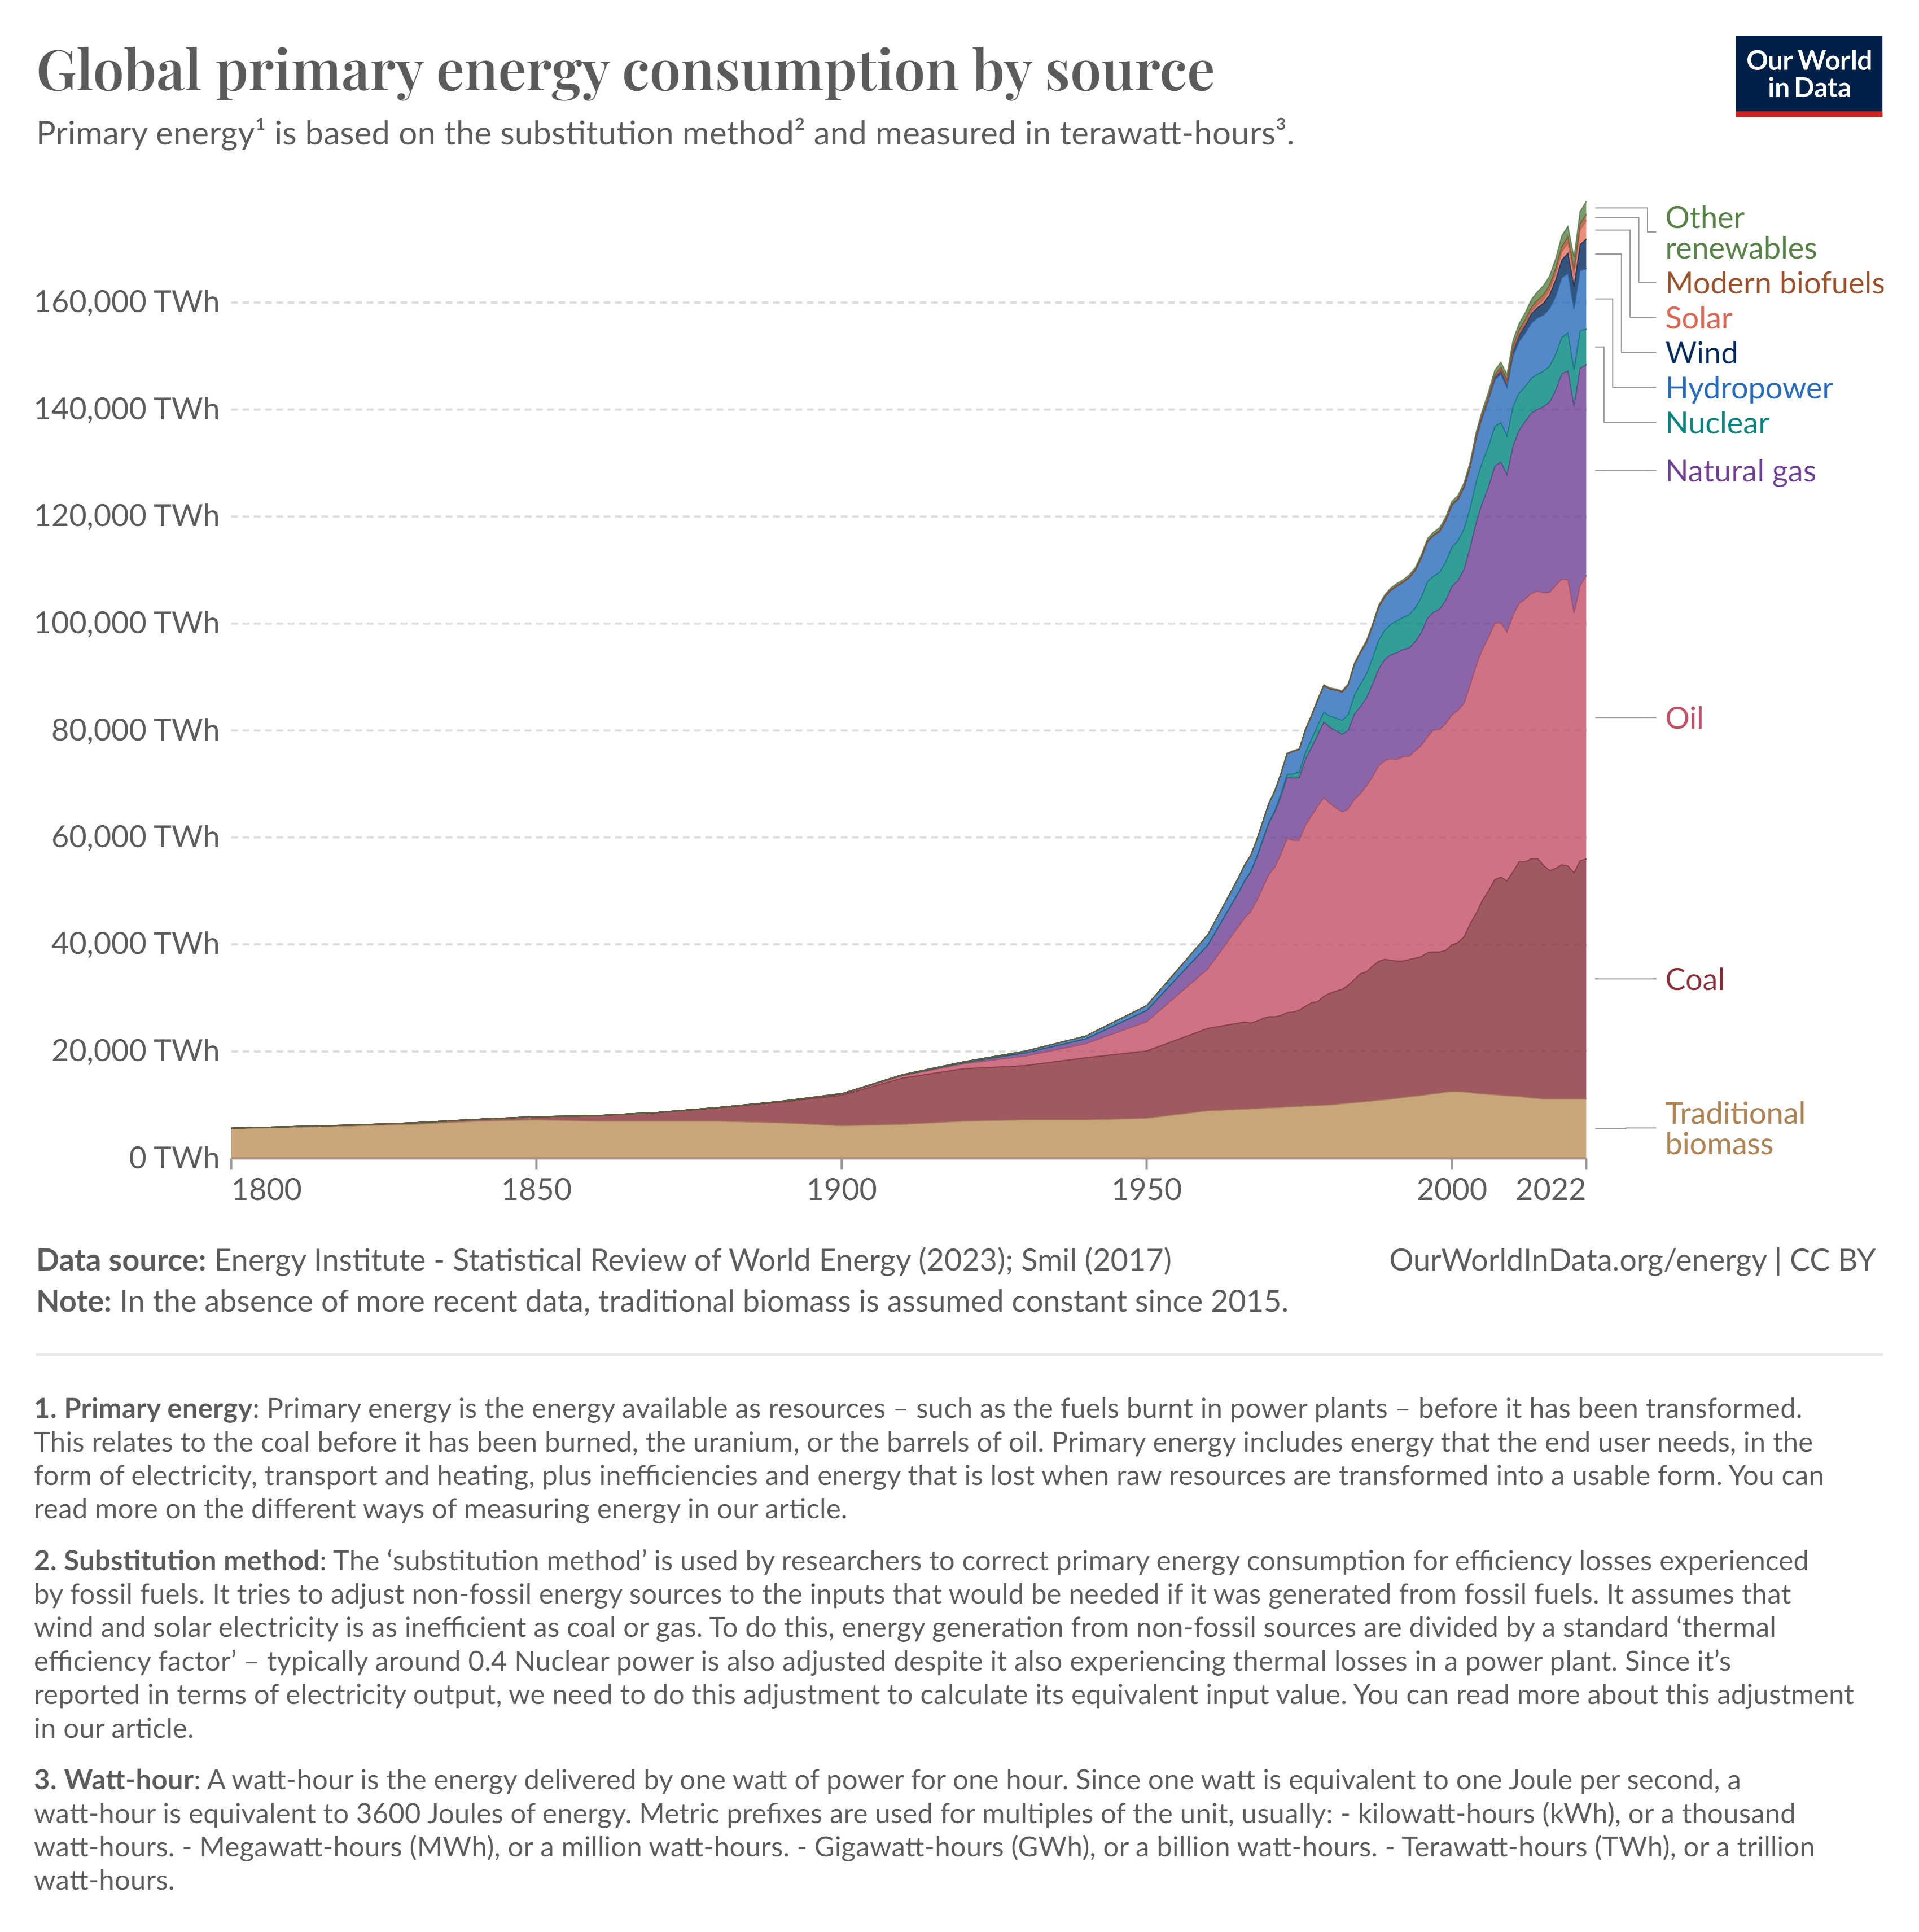
\includegraphics[width=0.8\textwidth]{global-energy-substitution.png}
\end{figure}

\section{Hyperscale Data Center Campus in the district “Rhein-Erfurt-Kreis”}


$\Rightarrow$  $\frac{200 \text{ MegaWatt}}{2} = 100 \times 10^6 \text{ Watt für Laptops}$\\
$\Rightarrow$  Anzahl Laptops = $\frac{100 \times 10^6 \text{ Watt}}{60 \text{ Watt pro Laptop}} = 1.67 \times 10^6$\\
$\Rightarrow$  Rechenleistung insgesamt = $1.67 \times 10^6 \times 100 \times 10^6\text{ FLOP/s} = 1.67 \times 10^{14} \text{ FLOP/s}$\\
$\Rightarrow$  Pro Minute = $1.67 \times 10^{14} \text{ FLOP/s} \times 60 \text{ s} = 1.0 \times 10^{16} \text{ FLOP}$\\
$\Rightarrow$  $1.0 \times 10^{16} = \frac{2}{3}n^3$\\
$\Rightarrow$  $n = \sqrt[3]{\frac{3}{2} \times 1.0 \times 10^{16}} = 246621.20743304683$\\\\
$n \approx 246621$
$\Rightarrow$  Dauer für einen Laptop = $\frac{1.0 \times 10^{16} \text{ FLOP}}{100 \times 10^6 \text{ FLOP/s}} = 1.0 \times 10^8 \text{ s} \approx 27777.78 \text{ h} = 1157.\overline{407} \text{ Tage}$\\

\section{connect to the cluster}
\begin{figure}[H]
    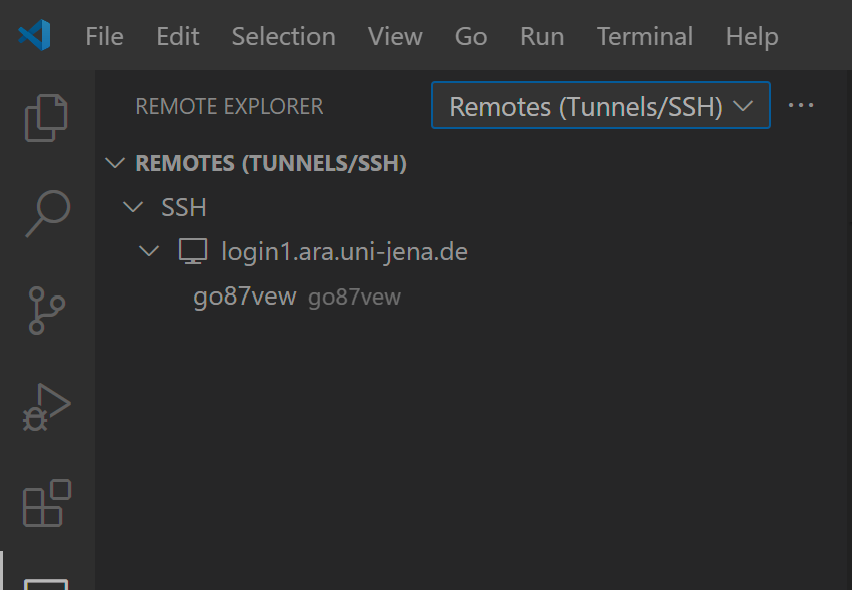
\includegraphics[width=0.8\textwidth]{ssh.png}
\end{figure}

\begin{figure}[H]
    
\includegraphics[width=0.8\textwidth]{cisco.png}
\end{figure}

\begin{figure}[H]
    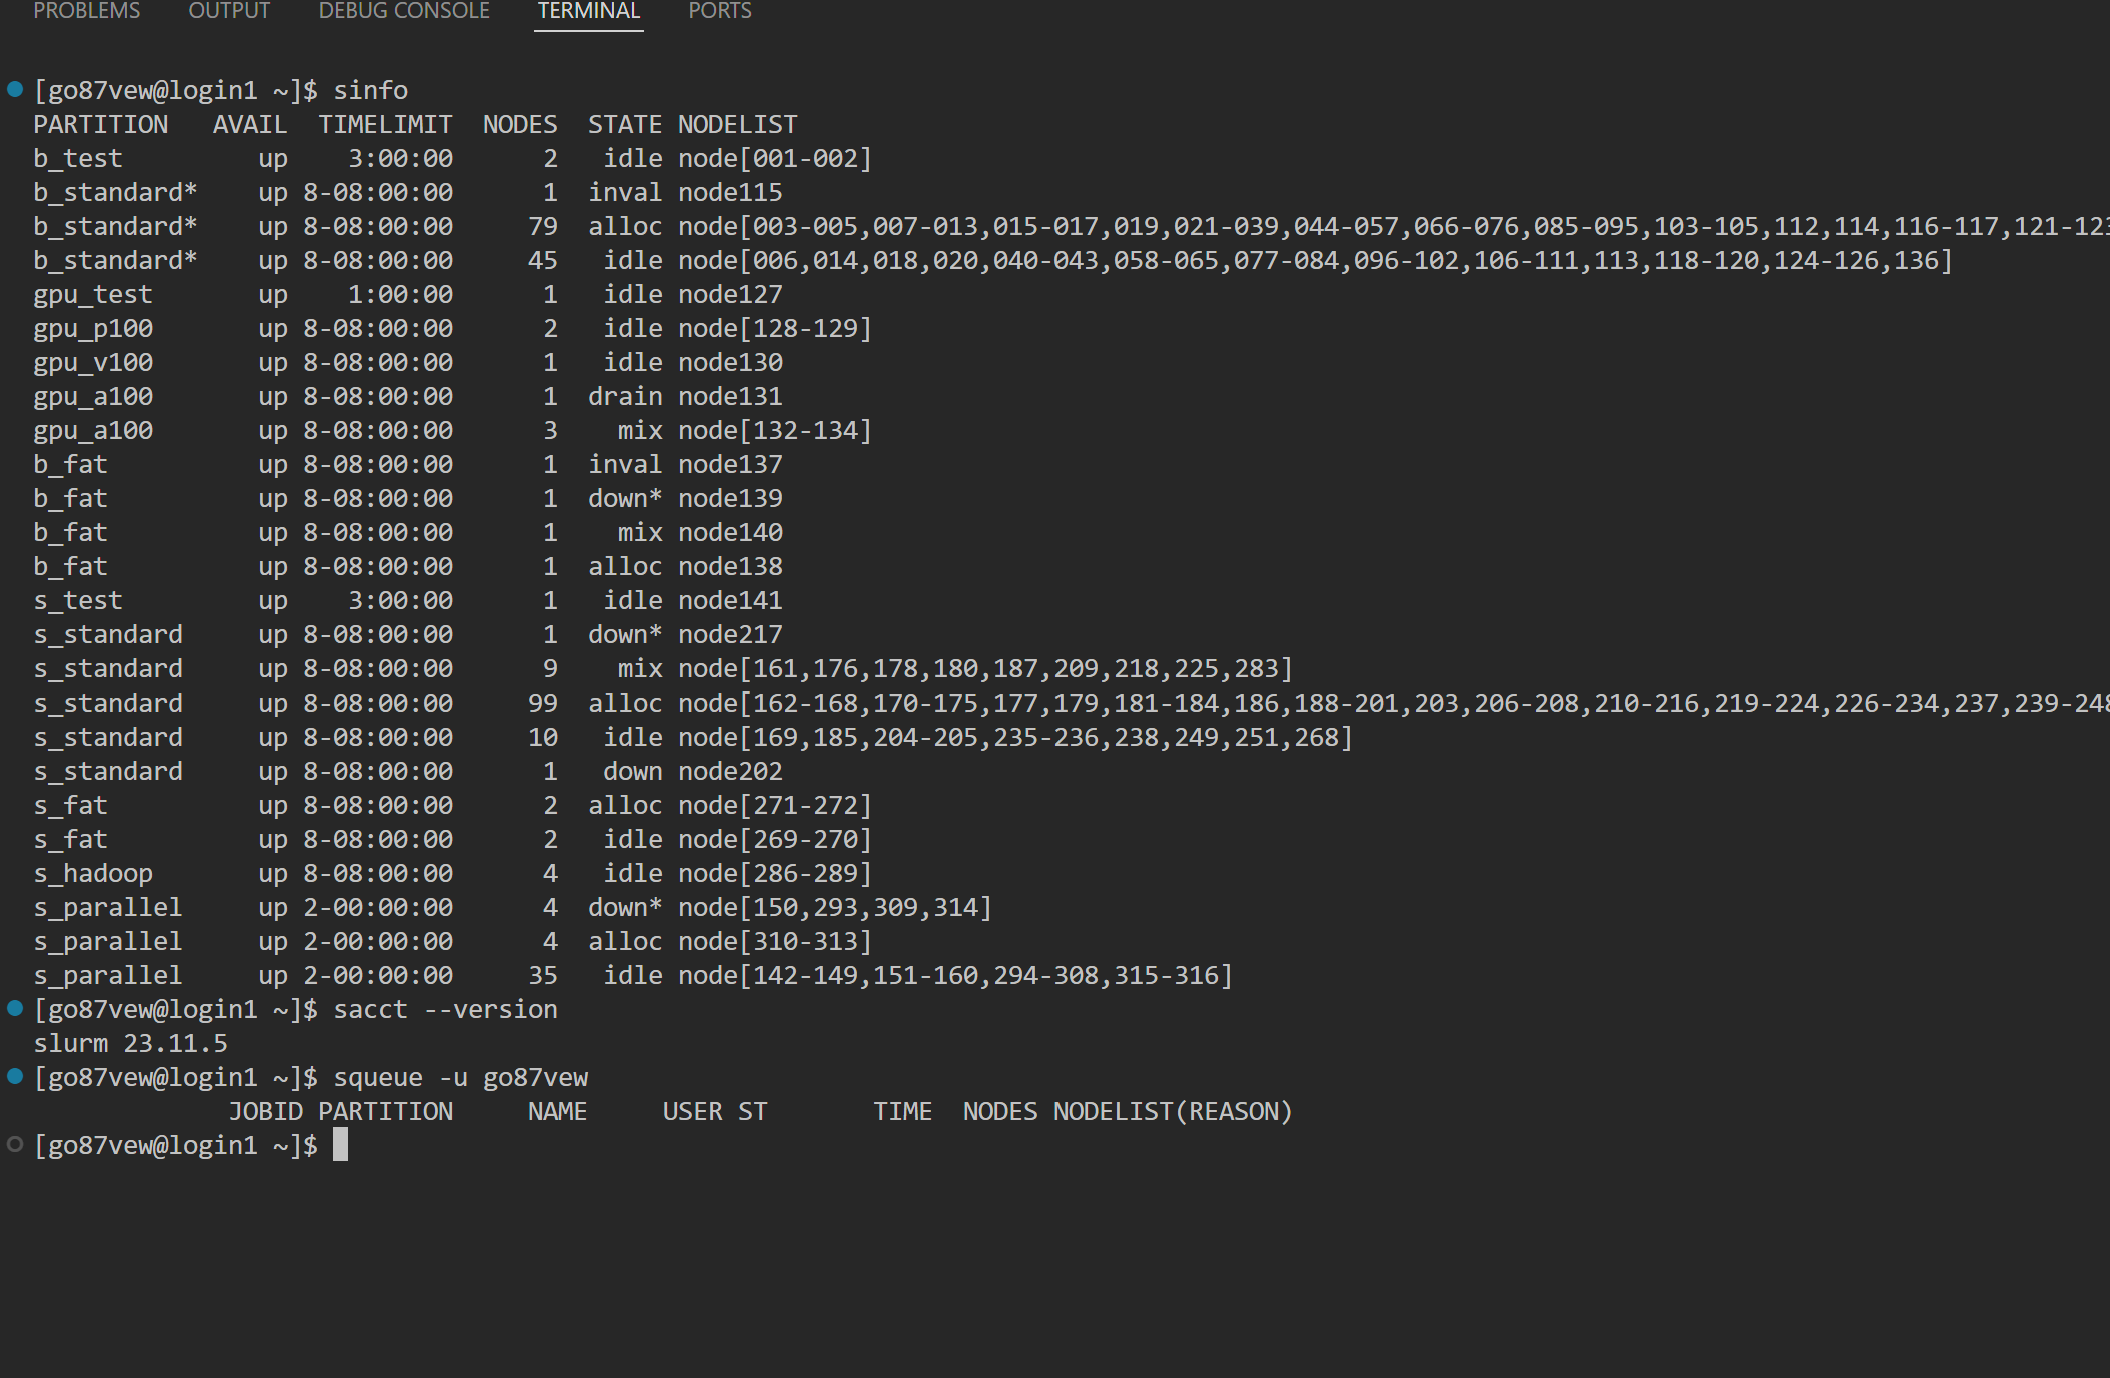
\includegraphics[width=0.7\textwidth]{ARA.png}
\end{figure}

\textbf{Mein altes sbatch Script für das Tsunami Lab.}

\begin{mdframed}[innertopmargin=0.2cm,
                 innerbottommargin= -0.5cm,
                 innerleftmargin=0.5cm, 
                 innerrightmargin=-5cm,
                 rightmargin=6cm]
    \begin{minted}{cpp}
    
    #!/bin/bash
    #SBATCH --job-name=tsunami
    #SBATCH --output=tsunami_output.txt
    #SBATCH --error=tsunami_error.txt
    #SBATCH --partition=s_hadoop
    #SBATCH --nodes=1
    #SBATCH --ntasks=1
    #SBATCH --time=180:00
    #SBATCH --cpus-per-task=72


    # Set the email address where notifications should be sent.
    #SBATCH --mail-user=daniel.schicker@uni-jena.de

    # Specify the types of email notifications you want to receive.
    #SBATCH --mail-type=BEGIN,END,FAIL

    # Load modules 
   module load tools/python/3.8
   module load compiler/gcc/11.2.0
   module load compiler/intel/2020-Update2
   module load libs/hdf5/1.10.8-gcc-10.2.0
   module load libs/zlib/1.2.11-intel-2018
   module load libs/netcdf/4.6.1-intel-2018
   python3.8 -m pip install --user scons

   date
   cd /beegfs/go87vew/tsunami_lab
   scons
   OMP_NUM_THREADS=32 ./build/tsunami_lab
   OMP_NUM_THREADS=34 ./build/tsunami_lab
   OMP_NUM_THREADS=36 ./build/tsunami_lab
  
    
    \end{minted}
\end{mdframed}

\end{document}
